\section{Data Description, Visualization and Statistical Analysis}

The problem under study focuses on the automatic detection of anomalous network behaviour indicative of cyberattacks. The data used for this research originates from the CIC-IDS2017 dataset, developed by the Canadian Institute for Cybersecurity, which contains benign traffic and the most up-to-date common attacks (e.g., DoS, DDoS, Brute Force, XSS, SQL Injection).

\subsection{Data Description}
The original dataset encompasses over 2.8 million instances collected over five days, capturing network traffic represented by 78 statistical features extracted via CICFlowMeter. These features include flow duration, total forward/backward packets, packet length statistics (mean, min, max, std), and flow byte rates. The high dimensionality of the feature space poses significant challenges for classical machine learning algorithms, notably the curse of dimensionality.

\subsection{Statistical Analysis and Quality Assessment}
Initial exploratory data analysis (EDA) identified several data quality issues inherent to raw network captures. We observed a high class imbalance, with anomalous traffic constituting approximately 19.7\% of the instances, while benign traffic represented the remaining 80.3\%. A visual representation of this distribution across our splits is shown in Figure \ref{fig:data_dist}.

Statistical profiling of the continuous variables revealed stark differences in magnitudes. For instance, the \texttt{Flow Duration} feature spans from a few microseconds to over 119 seconds, whereas \texttt{Packet Length} values are constrained to standard MTU limits (typically under 1500 bytes). This discrepancy necessitates robust scaling techniques.

\begin{figure}[ht]
    \centering
    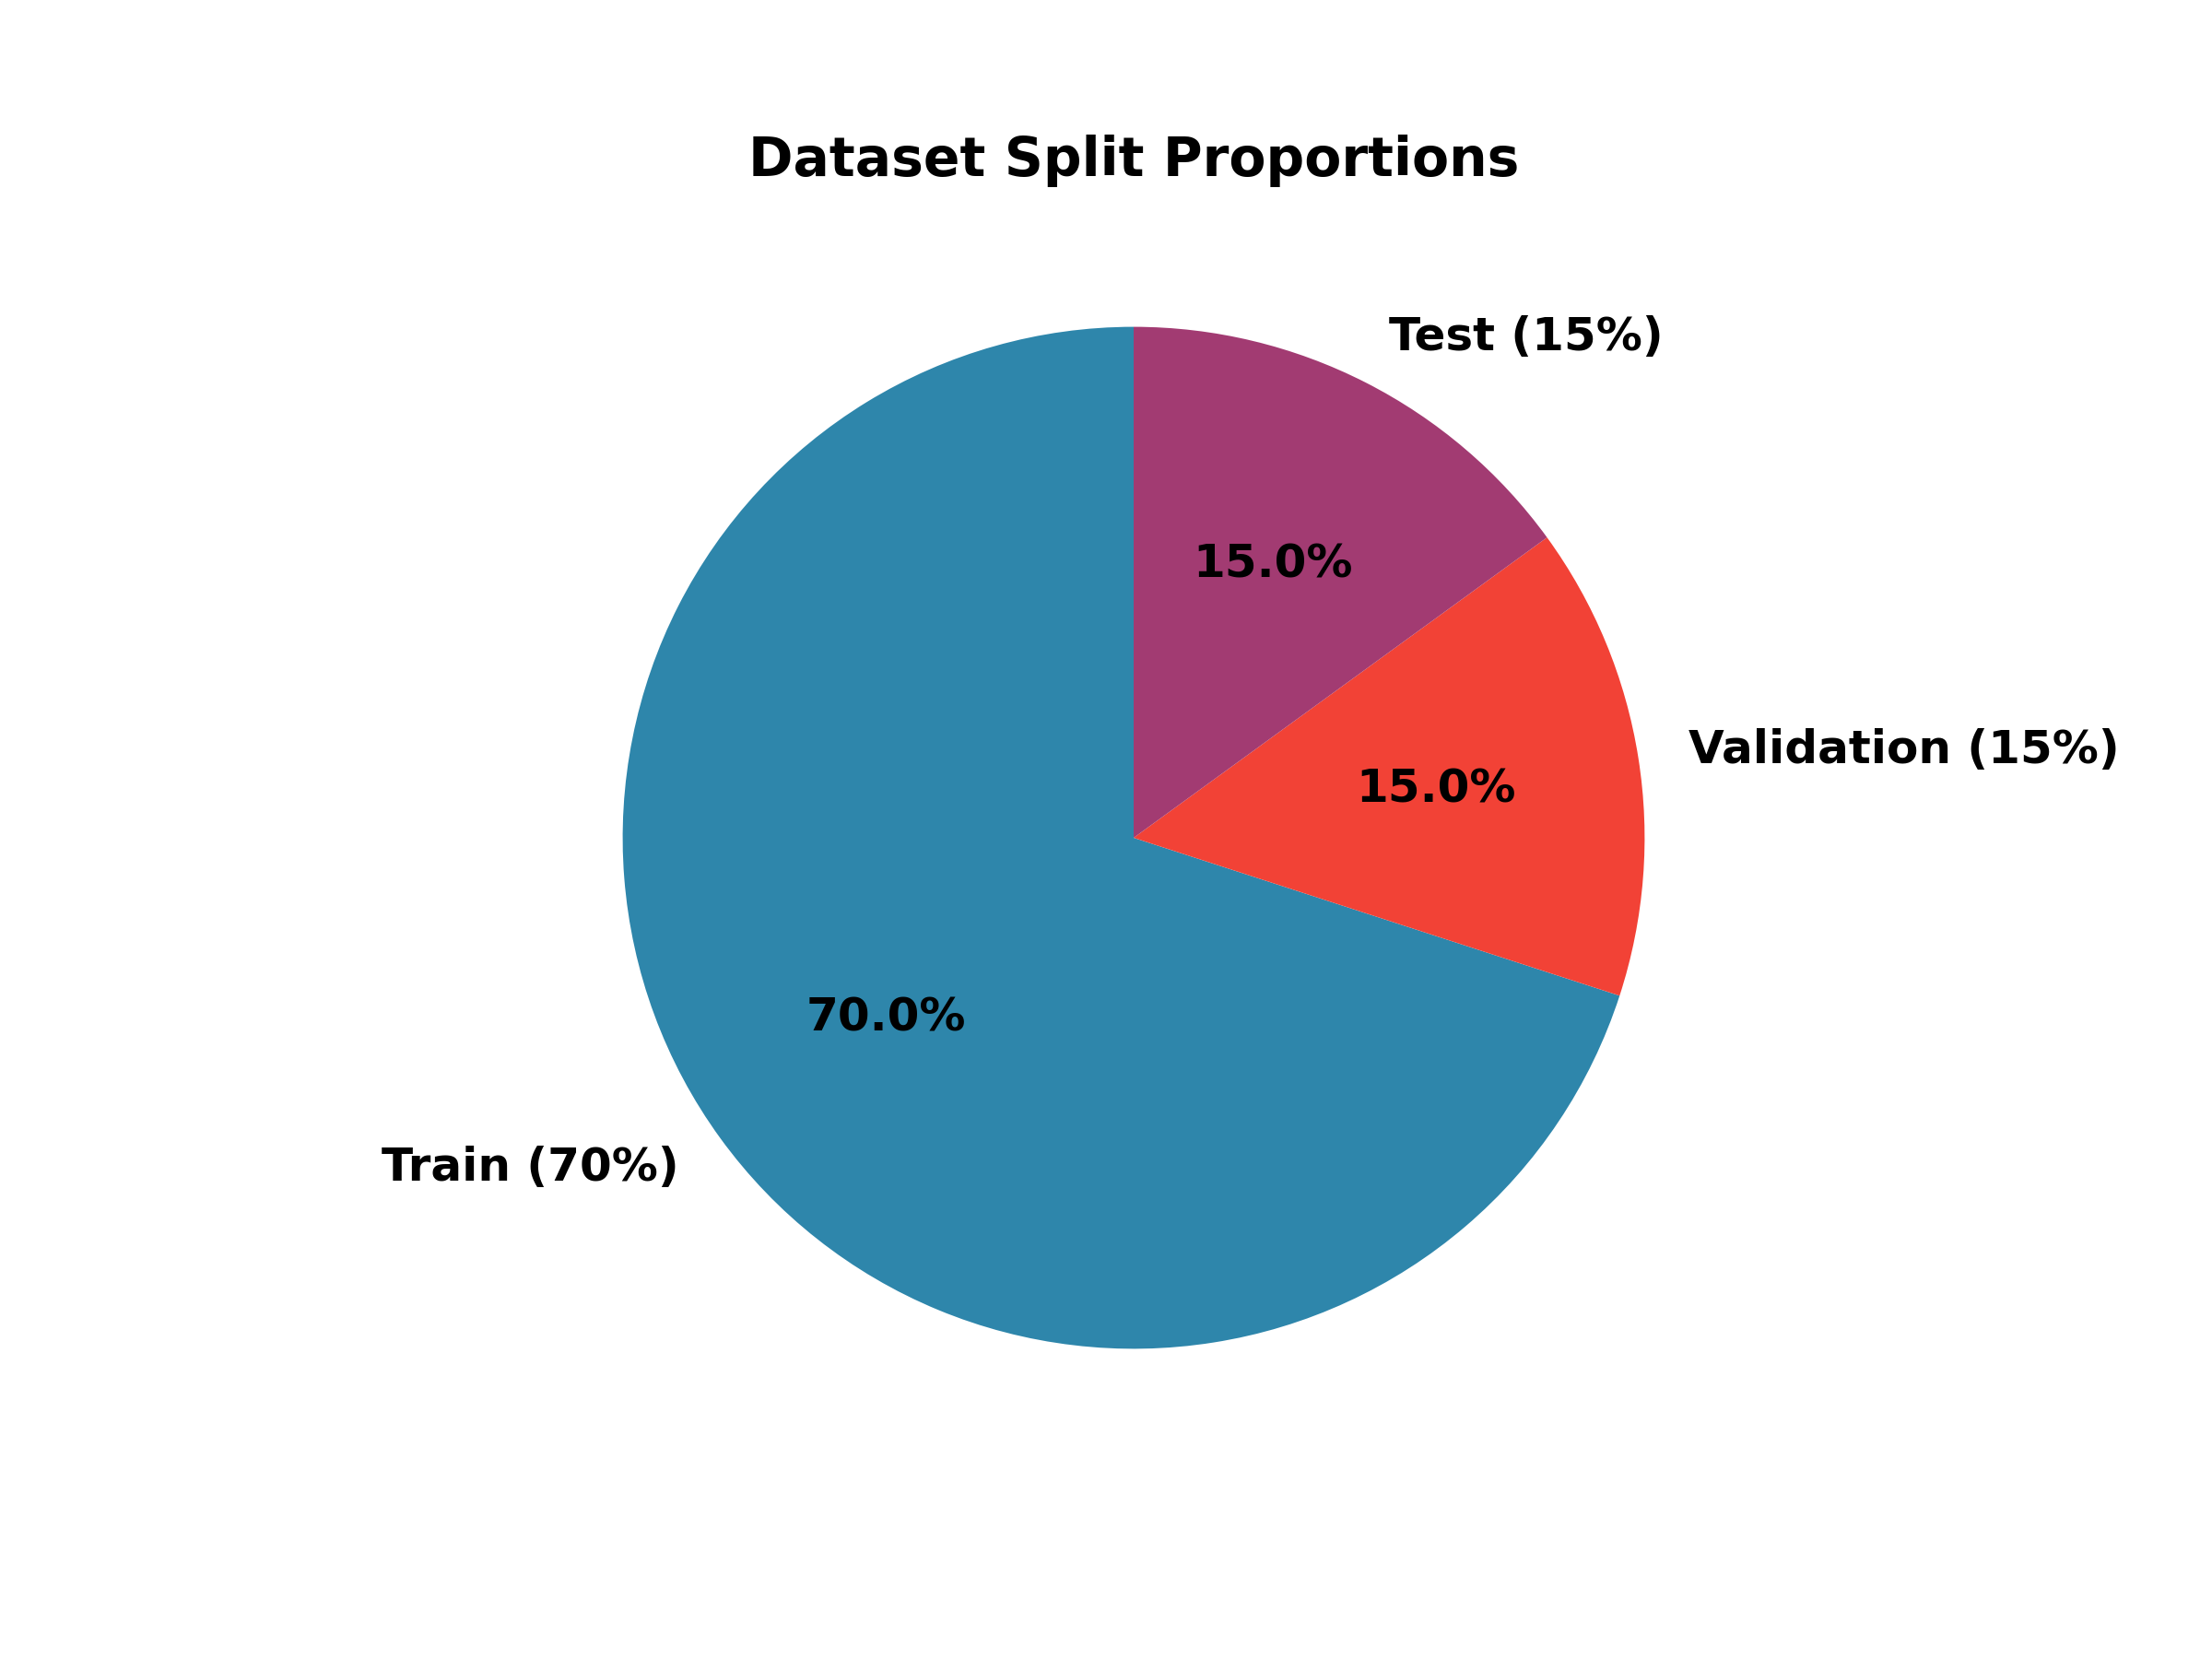
\includegraphics[width=0.48\columnwidth]{images/dataset_split.png}
    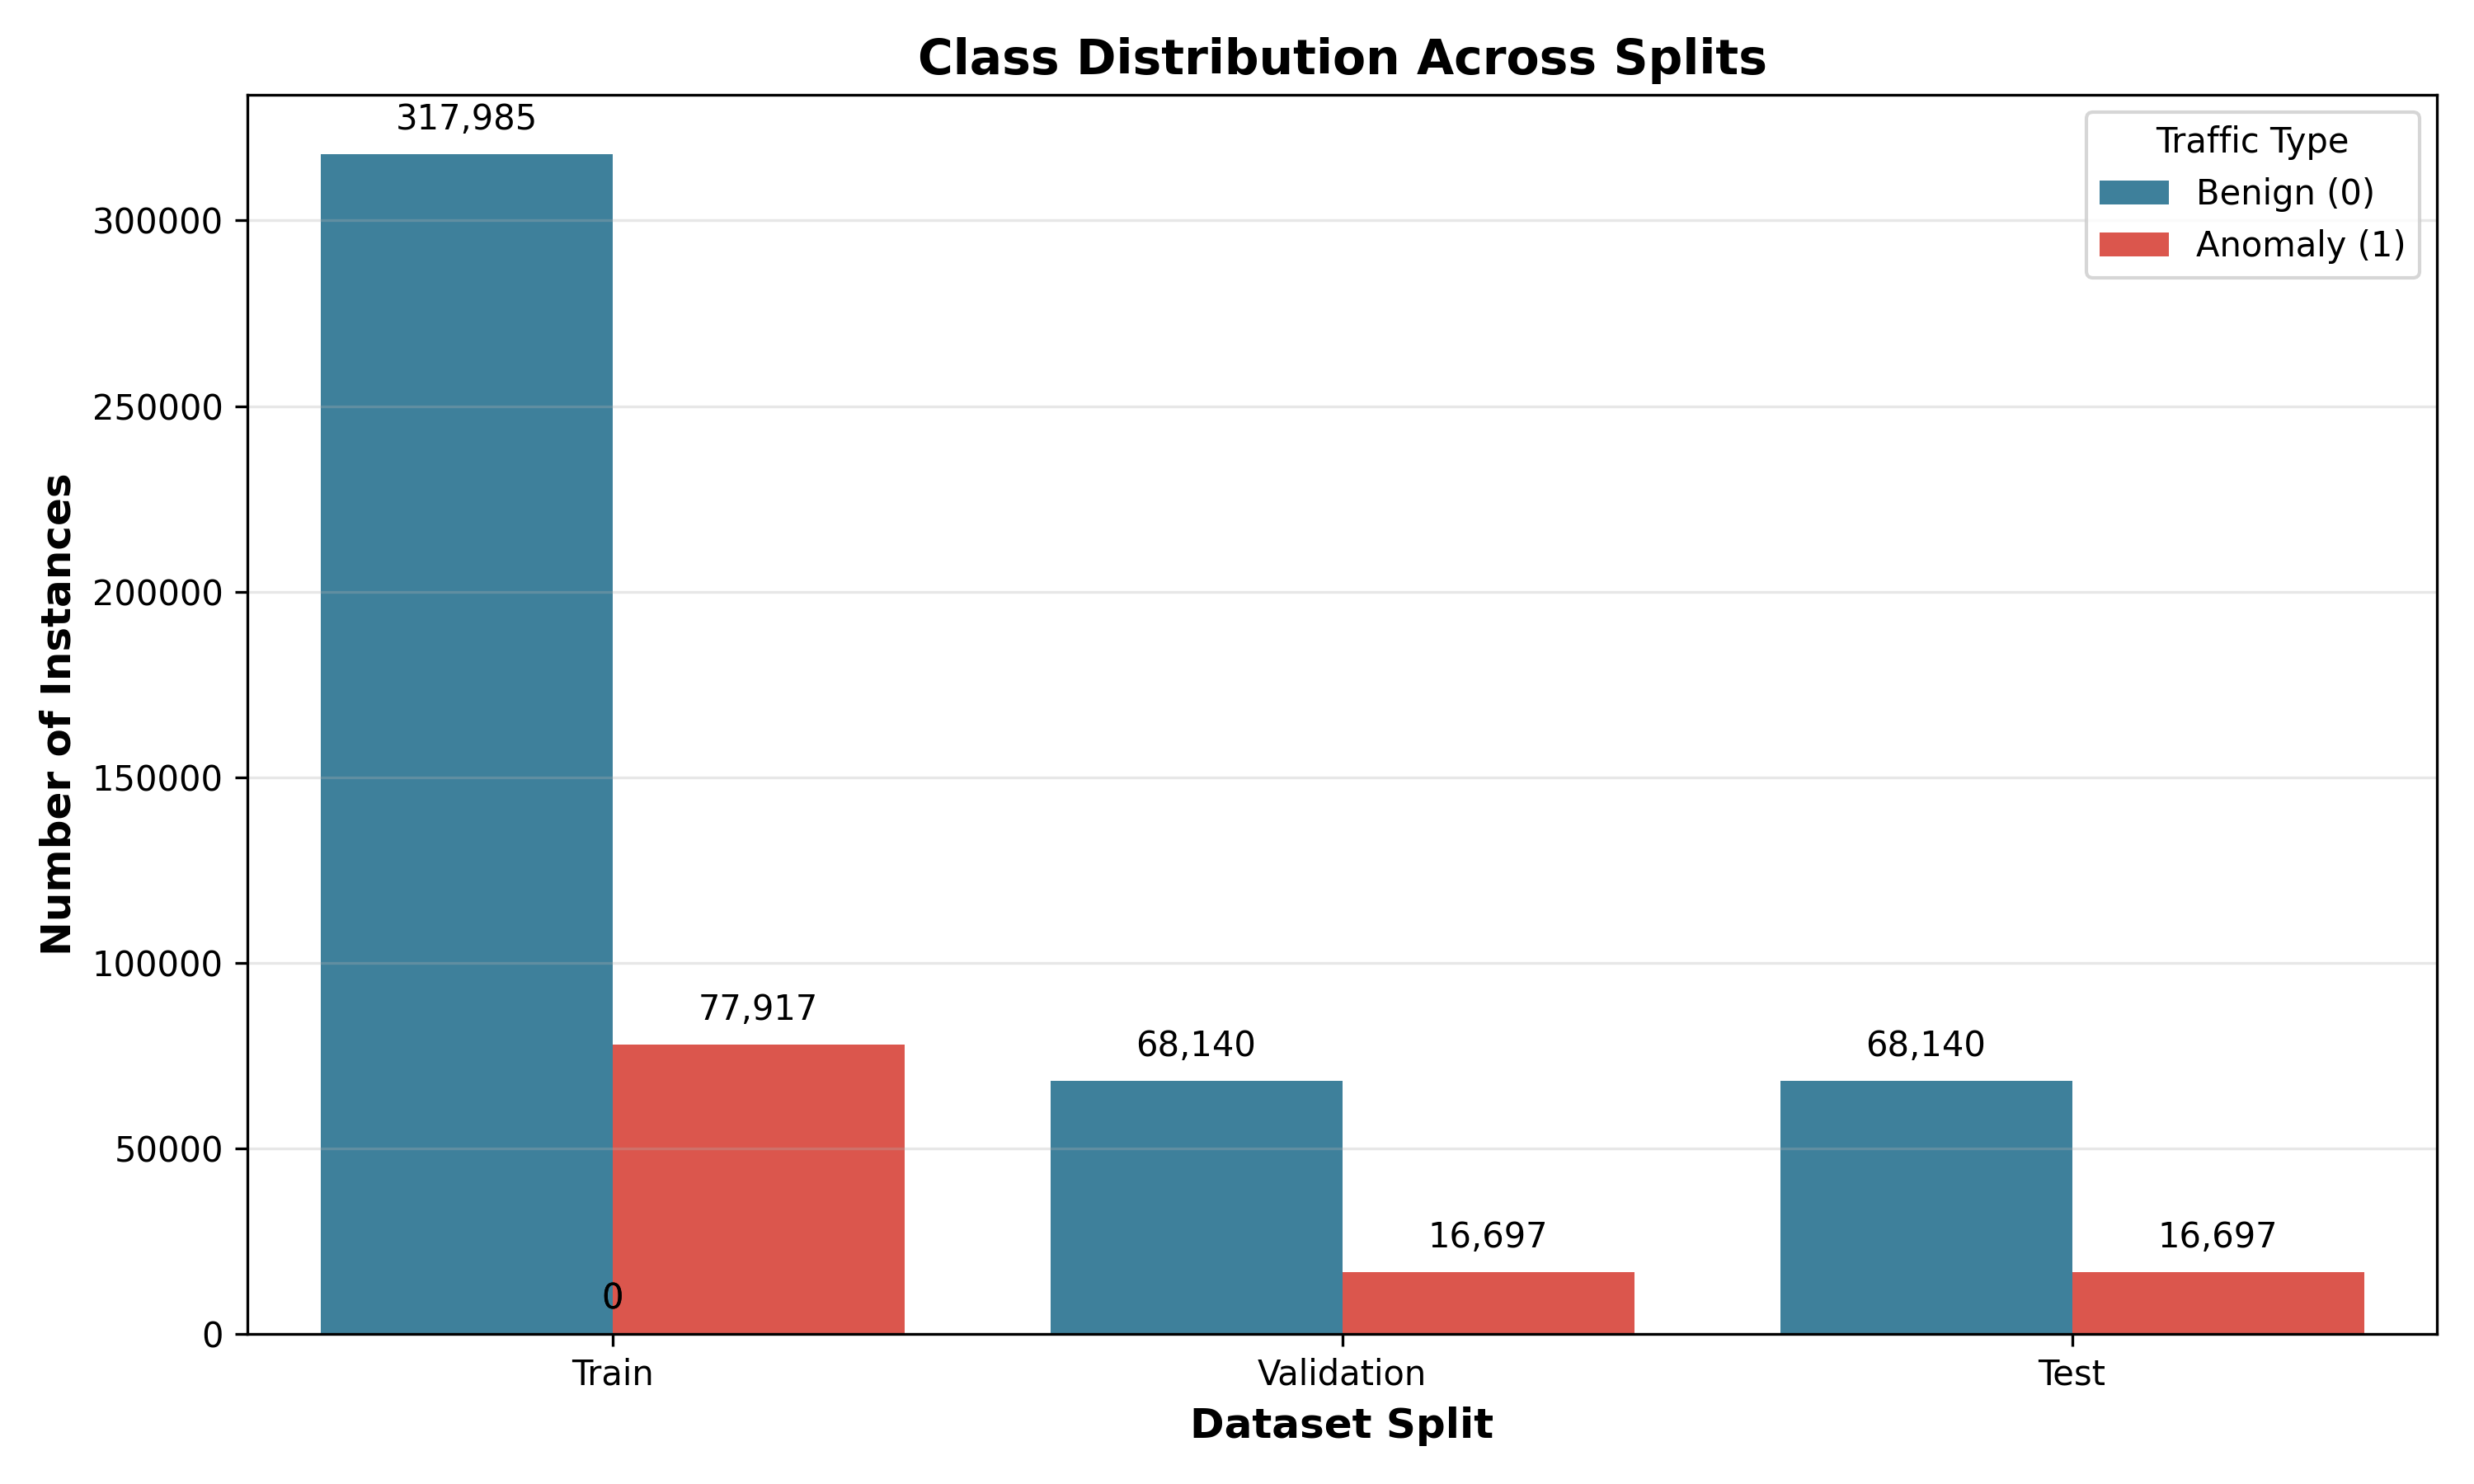
\includegraphics[width=0.48\columnwidth]{images/class_distribution.png}
    \caption{Dataset split proportions and class distribution across subsets.}
    \label{fig:data_dist}
\end{figure}

